\begin{figure}
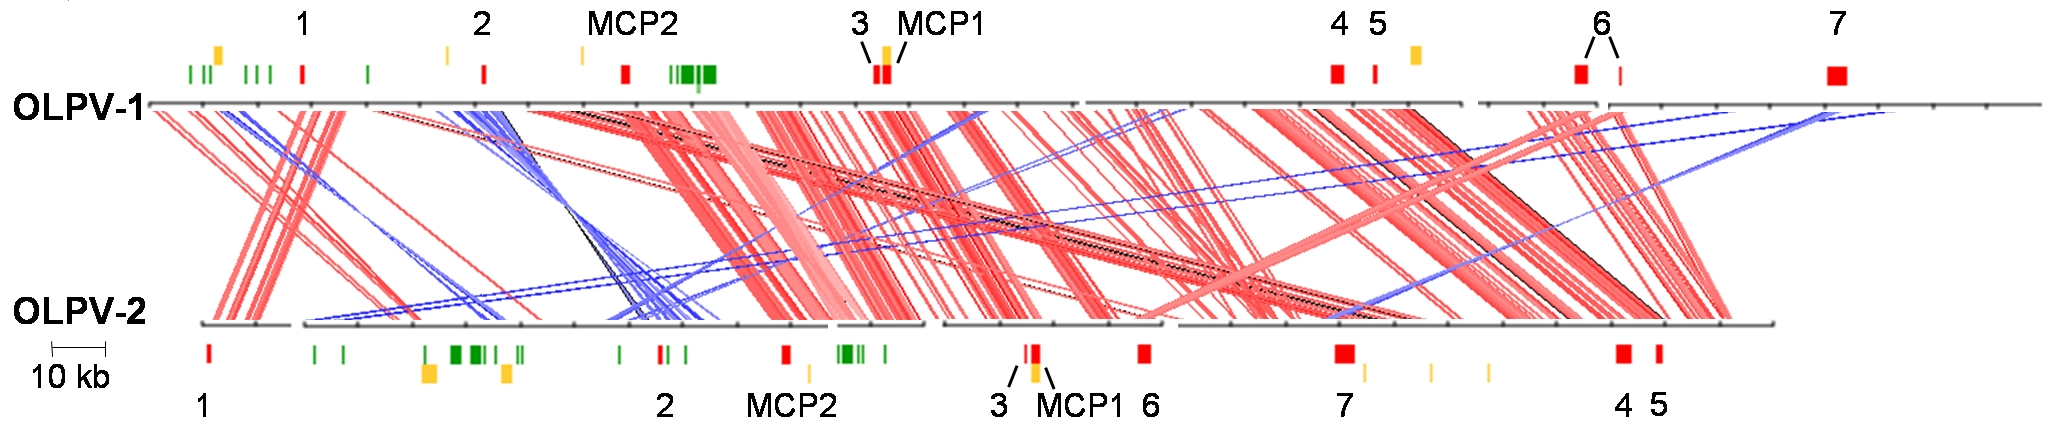
\includegraphics[width=\textwidth]{olv_figures/OLPV_genome.jpg}
\caption[Maps of \ac{OLPV} genomic scaffolds]{Maps of \ac{OLPV}-1 and \ac{OLPV}-2 scaffolds and comparison of the location of genes. Genes are marked as follows: single-copy conserved orthologues and \ac{MCP} (red), regions with identity to \ac{OLV} (green), proteins identified in the metaproteome (yellow), ribosomal nucleotide reductase \textbeta{} (1), VV A32 packaging ATPase (2), VV VLTF3 transcription factor (3), VV D5 replicative helicase (4), PbCV-1 A482R-like putative transcription factor (5), ribonucleotide reductase \textalpha{} (6), and \textsc{DNA} polymerase B (7). Lines connect homologous regions between the \ac{OLPV}-1 and \ac{OLPV}-2 scaffolds in the same orientation (red) and reverse orientation (blue).
}
\label{fig:OLPV_genome}

\end{figure}
